\documentclass[11pt]{article}
\usepackage[margin=1in]{geometry}
\usepackage{amsmath,amssymb,amsthm,mathtools,bm}
\usepackage{graphicx,booktabs,subcaption}
\usepackage[hidelinks]{hyperref}
\usepackage{enumitem}
\usepackage{xcolor}
\allowdisplaybreaks

\newtheorem{proposition}{Proposition}[section]
\newtheorem{theorem}[proposition]{Theorem}
\newtheorem{lemma}[proposition]{Lemma}
\newtheorem{remark}[proposition]{Remark}
\newtheorem{definition}[proposition]{Definition}

\newcommand{\R}{\mathbb{R}}
\newcommand{\E}{\mathbb{E}}
\newcommand{\Var}{\operatorname{Var}}
\newcommand{\Cov}{\operatorname{Cov}}
\newcommand{\diag}{\operatorname{diag}}
\newcommand{\tr}{\operatorname{tr}}
\newcommand{\Id}{I}
\newcommand{\trans}{\mathsf{T}}
\newcommand{\Ncal}{\mathcal{N}}
\newcommand{\norm}[1]{\left\lVert #1 \right\rVert}
\newcommand{\abs}[1]{\left| #1 \right|}

\title{Loss of Markovianity in Gaussian AR(1) Diffusion\\[2mm]
\large Precision fill-in, decay, and spectral interpretation}
\author{}
\date{}

\begin{document}
\maketitle

\begin{abstract}
A Gaussian AR(1) chain has a dense covariance but a tridiagonal precision. The tridiagonal pattern is the matrix form of Markov locality: conditionally on its neighbors, each frame is independent of the rest. After Ornstein--Uhlenbeck corruption,
\[
\Sigma_t=e^{-2t}\Sigma_0+(1-e^{-2t})\Id,
\qquad
S(x,t)=\nabla_x \log p_t(x)=-\Sigma_t^{-1}(x-\mu_t),
\]
so the full score structure is controlled by the noisy precision $Q_t:=\Sigma_t^{-1}$. This note derives $Q_0$ from first principles, shows explicitly that any $t>0$ produces nonzero long-range entries in $Q_t$, and explains the mechanism in two complementary ways. First, a Neumann expansion shows that diffusion fills the precision band one diagonal at a time. Second, a resolvent formula shows that $Q_t$ is a diagonal matrix minus the inverse of a tridiagonal matrix, hence dense with exponential off-diagonal decay. Numerical experiments for small and large dimension confirm the lifecycle
\[
\text{tridiagonal }Q_0 \longrightarrow \text{dense }Q_t \longrightarrow \Id\quad (t\to\infty).
\]
\end{abstract}

\section{Setup}
Let $N:=K+1$ and consider the Gaussian AR(1) recursion
\begin{equation}\label{eq:ar1}
 a_{k+1}=\alpha a_k+\eta_k,
 \qquad k=0,1,\dots,K-1,
\end{equation}
where $a_0\sim\Ncal(\mu_0,\sigma_0^2)$ and the innovations $\eta_k\sim\Ncal(0,\sigma_\eta^2)$ are independent of each other and of $a_0$. We collect the trajectory into the vector
\[
 a:=(a_0,a_1,\dots,a_K)^\trans\in\R^N.
\]
The mean is immediate from the recursion:
\[
\mu_k:=\E[a_k]=\alpha^k\mu_0,
\qquad
\mu_a:=(\mu_0,\alpha\mu_0,\dots,\alpha^K\mu_0)^\trans.
\]
For most structural statements the mean is irrelevant, so we work with the centered vector
\[
 c:=a-\mu_a.
\]

\section{The clean Gaussian law and its tridiagonal precision}
\subsection{Exact factorization of the quadratic form}
Define the innovation coordinates
\[
\xi_0:=c_0,
\qquad
\xi_k:=c_k-\alpha c_{k-1},\quad k=1,\dots,K.
\]
By construction,
\[
\xi_0=a_0-\mu_0,
\qquad
\xi_k=\eta_{k-1}\quad (k\ge 1),
\]
so the vector $\xi=(\xi_0,\dots,\xi_K)^\trans$ is Gaussian with independent coordinates and covariance
\[
D:=\diag(\sigma_0^2,\sigma_\eta^2,\dots,\sigma_\eta^2).
\]
Introduce the lower bidiagonal matrix
\[
L=
\begin{pmatrix}
1 & 0 & 0 & \cdots & 0 \\
-\alpha & 1 & 0 & \cdots & 0 \\
0 & -\alpha & 1 & \ddots & \vdots \\
\vdots & \ddots & \ddots & \ddots & 0 \\
0 & \cdots & 0 & -\alpha & 1
\end{pmatrix}.
\]
Then $\xi=Lc$. Since $\xi\sim\Ncal(0,D)$,
\[
p_0(a)
\propto
\exp\!\left(-\frac12\xi^\trans D^{-1}\xi\right)
=
\exp\!\left(-\frac12 c^\trans L^\trans D^{-1}L c\right).
\]
Therefore the clean precision is
\begin{equation}\label{eq:q0_factor}
Q_0:=\Sigma_0^{-1}=L^\trans D^{-1}L.
\end{equation}

\subsection{Expanding the entries of $Q_0$}
We now multiply out \eqref{eq:q0_factor} entry by entry.
\begin{proposition}[Explicit clean precision]\label{prop:q0}
The clean precision matrix is tridiagonal:
\begin{equation}\label{eq:q0_explicit}
Q_0=
\begin{pmatrix}
\sigma_0^{-2}+\alpha^2\sigma_\eta^{-2} & -\alpha\sigma_\eta^{-2} & 0 & \cdots & 0 \\
-\alpha\sigma_\eta^{-2} & (1+\alpha^2)\sigma_\eta^{-2} & -\alpha\sigma_\eta^{-2} & \ddots & \vdots \\
0 & -\alpha\sigma_\eta^{-2} & \ddots & \ddots & 0 \\
\vdots & \ddots & \ddots & (1+\alpha^2)\sigma_\eta^{-2} & -\alpha\sigma_\eta^{-2} \\
0 & \cdots & 0 & -\alpha\sigma_\eta^{-2} & \sigma_\eta^{-2}
\end{pmatrix}.
\end{equation}
\end{proposition}

\begin{proof}
Because $L$ has only one diagonal and one subdiagonal, $L^\trans D^{-1}L$ can only have one diagonal and one super/subdiagonal. We compute them explicitly.

For the $(1,1)$ entry only the first column of $L$ matters. It has nonzero entries $1$ in row $1$ and $-\alpha$ in row $2$, hence
\[
(Q_0)_{11}=\sigma_0^{-2}+\alpha^2\sigma_\eta^{-2}.
\]
For an interior diagonal entry $2\le i\le N-1$, the $i$th column of $L$ has entries $1$ in row $i$ and $-\alpha$ in row $i+1$, both weighted by $\sigma_\eta^{-2}$, so
\[
(Q_0)_{ii}=\sigma_\eta^{-2}+\alpha^2\sigma_\eta^{-2}=(1+\alpha^2)\sigma_\eta^{-2}.
\]
For the last diagonal entry only row $N$ contributes, giving
\[
(Q_0)_{NN}=\sigma_\eta^{-2}.
\]
Finally, for each neighboring pair $(i,i+1)$, the only common nonzero row in the $i$th and $(i+1)$th columns of $L$ is row $i+1$, where the entries are $-\alpha$ and $1$. Therefore
\[
(Q_0)_{i,i+1}=(Q_0)_{i+1,i}=-\alpha\sigma_\eta^{-2}.
\]
All other entries vanish because the corresponding columns of $L$ have disjoint support. This is exactly \eqref{eq:q0_explicit}.
\end{proof}

\subsection{Why this tridiagonal pattern is the Markov property}
For a Gaussian vector $X\sim\Ncal(\mu,\Sigma)$ with precision $Q=\Sigma^{-1}$, the conditional law of $X_i$ given all other coordinates is obtained by isolating all terms in the quadratic form that contain $x_i$:
\[
-\frac12 (x-\mu)^\trans Q(x-\mu)
= -\frac12 Q_{ii}(x_i-\mu_i)^2 - (x_i-\mu_i)\sum_{j\ne i}Q_{ij}(x_j-\mu_j) + \text{terms independent of }x_i.
\]
Completing the square gives
\begin{equation}\label{eq:cond_mean_general}
X_i\,\big|\,X_{-i}
\sim
\Ncal\!\left(
\mu_i-Q_{ii}^{-1}\sum_{j\ne i}Q_{ij}(X_j-\mu_j),
\;Q_{ii}^{-1}
\right).
\end{equation}
Hence $Q_{ij}=0$ means that $X_j$ does not enter the conditional mean of $X_i$ once the other coordinates are known. For Gaussian vectors this is exactly conditional independence.

Applying \eqref{eq:cond_mean_general} to $Q_0$ in \eqref{eq:q0_explicit}, every interior coordinate $a_k$ depends conditionally only on $a_{k-1}$ and $a_{k+1}$. In the stationary zero-mean case $\sigma_0^2=\sigma_\eta^2/(1-\alpha^2)$ this becomes especially transparent:
\begin{equation}\label{eq:cond_mean_stationary}
\E[a_k\mid a_{-k}]
=
\frac{\alpha}{1+\alpha^2}(a_{k-1}+a_{k+1}),
\qquad
\Var(a_k\mid a_{-k})=\frac{\sigma_\eta^2}{1+\alpha^2},
\qquad 1\le k\le K-1.
\end{equation}
So the sparsity of $Q_0$ is not a secondary fact. It is the algebraic form of Markov locality.

\section{OU diffusion: covariance and score}
Let $z\sim\Ncal(0,\Id_N)$ be independent of $a$, and define the noisy observation
\begin{equation}\label{eq:xt_def}
 x=e^{-t}a+\sqrt{\Delta_t}\,z,
 \qquad
 \Delta_t:=1-e^{-2t},
 \qquad
 \beta_t:=e^{-2t}.
\end{equation}
Then
\begin{equation}\label{eq:mut}
\mu_t:=\E[x]=e^{-t}\mu_a,
\end{equation}
and, because $a$ and $z$ are independent,
\begin{equation}\label{eq:sigmat}
\Sigma_t:=\Cov(x)=\beta_t\Sigma_0+\Delta_t\Id.
\end{equation}
Since $x$ is Gaussian, its log-density is quadratic and its score is affine:
\begin{equation}\label{eq:score_gaussian}
S(x,t)=\nabla_x\log p_t(x)=-Q_t(x-\mu_t),
\qquad
Q_t:=\Sigma_t^{-1}.
\end{equation}
The entire question is therefore: \emph{what happens to the matrix $Q_t$?}

\section{The first nonzero long-range entry: a three-frame calculation}
Take the stationary zero-mean case and set $N=3$. Then
\[
\Sigma_0=\sigma_\infty^2
\begin{pmatrix}
1 & \alpha & \alpha^2 \\
\alpha & 1 & \alpha \\
\alpha^2 & \alpha & 1
\end{pmatrix},
\qquad
\sigma_\infty^2=\frac{\sigma_\eta^2}{1-\alpha^2}.
\]
Write
\[
 u:=\Delta_t+\beta_t\sigma_\infty^2,
 \qquad
 v:=\beta_t\sigma_\infty^2\alpha,
 \qquad
 w:=\beta_t\sigma_\infty^2\alpha^2.
\]
Then
\[
\Sigma_t=
\begin{pmatrix}
 u & v & w \\
 v & u & v \\
 w & v & u
\end{pmatrix}.
\]
The $(1,3)$ entry of the inverse is the corresponding cofactor divided by $\det\Sigma_t$:
\begin{equation}\label{eq:13cofactor}
(Q_t)_{13}=\frac{v^2-uw}{\det\Sigma_t}.
\end{equation}
Now compute the numerator explicitly:
\[
 v^2-uw
 = \beta_t^2\sigma_\infty^4\alpha^2 - (\Delta_t+\beta_t\sigma_\infty^2)(\beta_t\sigma_\infty^2\alpha^2)
 = -\beta_t\Delta_t\sigma_\infty^2\alpha^2.
\]
Therefore
\begin{equation}\label{eq:q13_explicit}
(Q_t)_{13}=-\frac{\beta_t\Delta_t\sigma_\infty^2\alpha^2}{\det\Sigma_t}.
\end{equation}
For every $t>0$ and every $\alpha\ne 0$, the denominator is positive because $\Sigma_t$ is positive definite, while the numerator is strictly negative. Hence
\[
(Q_t)_{13}\ne 0\qquad (t>0).
\]
At $t=0$ this entry is exactly zero; the instant diffusion begins, the zero is filled.

\section{Mechanism of fill-in: two exact matrix identities}
\subsection{Small-time band generation}
Starting from \eqref{eq:sigmat}, factor out $\beta_t$:
\[
\Sigma_t=\beta_t\big(\Sigma_0+c_t\Id\big),
\qquad
c_t:=e^{2t}-1=\frac{\Delta_t}{\beta_t}.
\]
Since $\Sigma_0=Q_0^{-1}$,
\[
\Sigma_t=\beta_t Q_0^{-1}(\Id+c_tQ_0),
\]
so
\begin{equation}\label{eq:qt_neumann_identity}
Q_t=e^{2t}(\Id+c_tQ_0)^{-1}Q_0.
\end{equation}
If $c_t\norm{Q_0}<1$, then the Neumann series converges:
\begin{equation}\label{eq:qt_neumann}
Q_t=e^{2t}\sum_{m=0}^{\infty}(-c_t)^mQ_0^{m+1}.
\end{equation}
This formula explains the fill-in mechanically. Because $Q_0$ is tridiagonal, $Q_0^{m+1}$ has bandwidth $m+1$. Therefore:
\begin{itemize}[leftmargin=1.5em]
\item $m=0$ contributes the original tridiagonal matrix $Q_0$;
\item $m=1$ adds the second off-diagonal band;
\item $m=2$ adds the third off-diagonal band;
\item and so on.
\end{itemize}
Diffusion does not destroy locality in one jump. It adds longer and longer conditional paths order by order.

\subsection{Exact resolvent form}
There is a second identity, valid for all $t>0$ and more useful globally. Write \eqref{eq:sigmat} as
\[
\Sigma_t=\Delta_t(\Id+\gamma_t\Sigma_0),
\qquad
\gamma_t:=\frac{\beta_t}{\Delta_t}.
\]
Then
\begin{equation}\label{eq:qt_gamma}
Q_t=\frac{1}{\Delta_t}(\Id+\gamma_t\Sigma_0)^{-1}.
\end{equation}
Since $\Id+\gamma_t\Sigma_0=Q_0^{-1}(Q_0+\gamma_t\Id)$,
\[
(\Id+\gamma_t\Sigma_0)^{-1}=(Q_0+\gamma_t\Id)^{-1}Q_0,
\]
and therefore
\begin{equation}\label{eq:qt_resolvent}
Q_t=\frac{1}{\Delta_t}\Big[\Id-\gamma_t(Q_0+\gamma_t\Id)^{-1}\Big].
\end{equation}
So every off-diagonal entry of $Q_t$ comes from the inverse of the tridiagonal matrix $B_t:=Q_0+\gamma_t\Id$.

\begin{proposition}[Every off-diagonal entry becomes nonzero]\label{prop:all_nonzero}
Fix $t>0$ and assume $\alpha\ne 0$. Then every off-diagonal entry of $Q_t$ is nonzero.
\end{proposition}

\begin{proof}
Write $b:=\alpha\sigma_\eta^{-2}>0$ and index matrices from $1$ to $N$. The matrix $B_t$ is tridiagonal with positive diagonal entries $d_1,\dots,d_N$ and constant off-diagonals $-b$. Define the leading and trailing determinant recursions
\[
\theta_0=1,
\qquad
\theta_1=d_1,
\qquad
\theta_k=d_k\theta_{k-1}-b^2\theta_{k-2}
\quad (k\ge 2),
\]
\[
\phi_{N+1}=1,
\qquad
\phi_N=d_N,
\qquad
\phi_k=d_k\phi_{k+1}-b^2\phi_{k+2}
\quad (k\le N-1).
\]
Because $B_t$ is symmetric positive definite, all principal minors are positive, hence all $\theta_k$ and $\phi_k$ are positive. The explicit inverse formula for a tridiagonal matrix gives, for $i<j$,
\[
(B_t^{-1})_{ij}=b^{j-i}\frac{\theta_{i-1}\phi_{j+1}}{\theta_N}>0.
\]
Using \eqref{eq:qt_resolvent},
\[
(Q_t)_{ij}=-\frac{\gamma_t}{\Delta_t}(B_t^{-1})_{ij}<0
\qquad (i\ne j).
\]
So no off-diagonal entry can vanish.
\end{proof}

\section{Quantifying the loss of locality}
\subsection{Finite-$N$ metrics}
For any matrix $M\in\R^{N\times N}$ and any radius $r\ge 1$, define the off-diagonal band share
\begin{equation}\label{eq:Rr_def}
R_r(M):=
\frac{\sum_{1\le \abs{i-j}\le r}\abs{M_{ij}}}{\sum_{i\ne j}\abs{M_{ij}}}.
\end{equation}
We use it on $M=Q_t$ and write $R_r(t):=R_r(Q_t)$. Then:
\begin{itemize}[leftmargin=1.5em]
\item $R_1(0)=1$ because $Q_0$ is exactly tridiagonal;
\item $R_1(t)<1$ for every $t>0$ by Proposition~\ref{prop:all_nonzero};
\item as $t\to\infty$, all off-diagonal entries vanish and $Q_t\to\Id$, so the total coupling strength goes to zero.
\end{itemize}
Thus the lifecycle is not monotone. Diffusion first creates longer-range conditional couplings, then eventually erases all couplings as isotropic noise dominates.

A second useful diagnostic is the distance profile
\begin{equation}\label{eq:Cd_def}
C_d(t):=
\frac{1}{\#\{(i,j):\abs{i-j}=d\}}
\sum_{\abs{i-j}=d}\abs{(Q_t)_{ij}},
\qquad d=1,2,\dots,N-1.
\end{equation}
This measures how strongly the precision couples coordinates at graph distance $d$.

\subsection{Stationary infinite-chain formula}
For a clean stationary chain the covariance is Toeplitz,
\[
(\Sigma_0)_{ij}=\sigma_\infty^2\alpha^{\abs{i-j}},
\qquad
\sigma_\infty^2=\frac{\sigma_\eta^2}{1-\alpha^2},
\]
and the interior precision symbol is
\[
q_0(\theta)=\frac{1+\alpha^2-2\alpha\cos\theta}{\sigma_\eta^2}.
\]
After diffusion,
\begin{equation}\label{eq:qt_symbol}
q_t(\theta)=\frac{1}{\beta_t\sigma_\eta^2/(1+\alpha^2-2\alpha\cos\theta)+\Delta_t}
=
\frac{1+\alpha^2-2\alpha\cos\theta}{\beta_t\sigma_\eta^2+\Delta_t(1+\alpha^2-2\alpha\cos\theta)}.
\end{equation}
At $t=0$, this is a first-degree trigonometric polynomial in $\cos\theta$, so its Fourier coefficients vanish beyond distance $1$: that is exactly the tridiagonal precision. For every $t>0$, the denominator depends on $\cos\theta$, so $q_t$ is a rational function and its Fourier series contains all harmonics. That is the spectral version of fill-in.

The same statement can be written directly in physical space. Let
\[
a_t:=1+\alpha^2+\gamma_t\sigma_\eta^2,
\qquad
\rho_t:=\frac{a_t-\sqrt{a_t^2-4\alpha^2}}{2\alpha}
\qquad (0<\rho_t<1,\;0<\alpha<1).
\]
Then the inverse of the infinite tridiagonal resolvent has Green's function
\[
(Q_0+\gamma_t\Id)^{-1}_{ij}
=
\frac{\sigma_\eta^2}{\sqrt{a_t^2-4\alpha^2}}\,\rho_t^{\abs{i-j}},
\]
and \eqref{eq:qt_resolvent} gives, for $i\ne j$,
\begin{equation}\label{eq:qt_geometric}
(Q_t)_{ij}=-A_t\rho_t^{\abs{i-j}},
\qquad
A_t:=\frac{\gamma_t\sigma_\eta^2}{\Delta_t\sqrt{a_t^2-4\alpha^2}}.
\end{equation}
So diffusion does \emph{not} produce arbitrary dense structure. It produces a dense matrix with controlled exponential decay.

In this idealized translation-invariant setting, the off-diagonal band share has the closed form
\begin{equation}\label{eq:Rr_rho}
R_r^{(\infty)}(t)=
\frac{\sum_{d=1}^r \rho_t^d}{\sum_{d=1}^{\infty}\rho_t^d}
=1-\rho_t^r.
\end{equation}
Larger $\rho_t$ means weaker locality.

\section{Spectral interpretation: which cancellation is broken?}
For finite $N$, diagonalize the clean covariance as
\[
\Sigma_0=U\Lambda U^\trans,
\qquad
\Lambda=\diag(\lambda_1,\dots,\lambda_N),
\qquad
U^\trans U=\Id.
\]
Then
\begin{equation}\label{eq:qt_spectral}
Q_t=U\,\diag\!\left(\frac{1}{\beta_t\lambda_1+\Delta_t},\dots,\frac{1}{\beta_t\lambda_N+\Delta_t}\right)U^\trans.
\end{equation}
At $t=0$ the weights are $1/\lambda_m$. Their particular values cause exact cancellations among the dense rank-one matrices $u_m u_m^\trans$, and the result is the tridiagonal matrix $Q_0$. Once diffusion changes the weights to $(\beta_t\lambda_m+\Delta_t)^{-1}$, those exact cancellations no longer hold. The matrix becomes full.

This also explains the late-time limit. As $t\to\infty$, all weights tend to $1$, so \eqref{eq:qt_spectral} tends to $U\Id U^\trans=\Id$. The endpoint is not ``long-range Markov''; it is \emph{no coupling at all}. Diffusion first breaks local conditional structure, then washes out structure entirely.

\section{Numerical experiments}
All figures were generated by the reproducible script \texttt{code/generate\_figures.py}. We used the stationary choice $\alpha=0.88$, $\sigma_\eta^2=1-\alpha^2$, hence $\sigma_\infty^2=1$.

\begin{figure}[ht!]
\centering
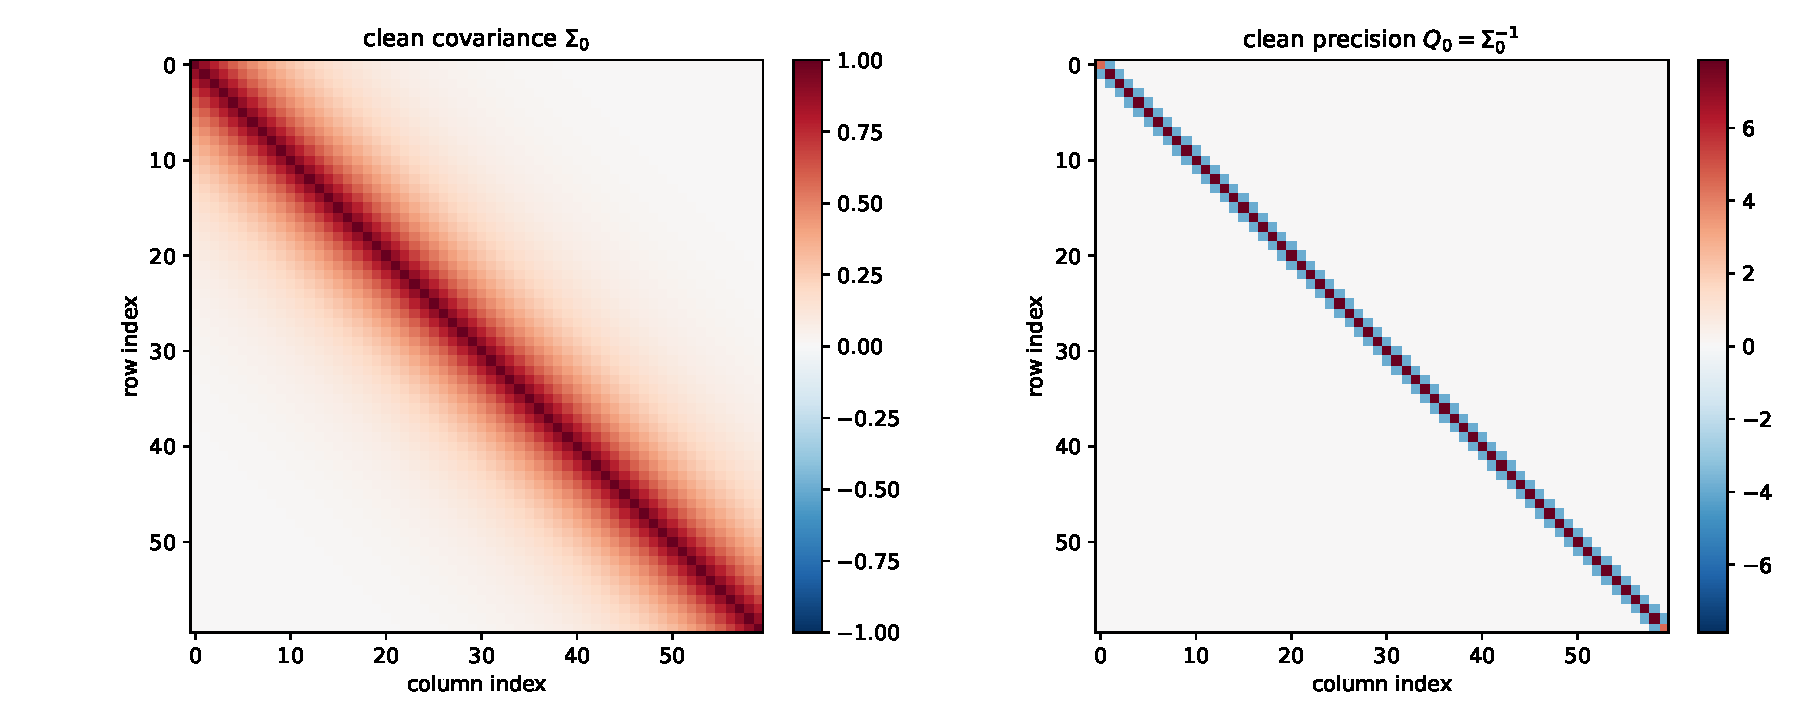
\includegraphics[width=.9\textwidth]{figures/fig01_cov_vs_prec.pdf}
\caption{Clean covariance versus clean precision for $N=60$. The covariance is dense because marginal correlations propagate through the recursion. The precision is tridiagonal because conditional dependence is local.}
\end{figure}

\begin{figure}[ht!]
\centering
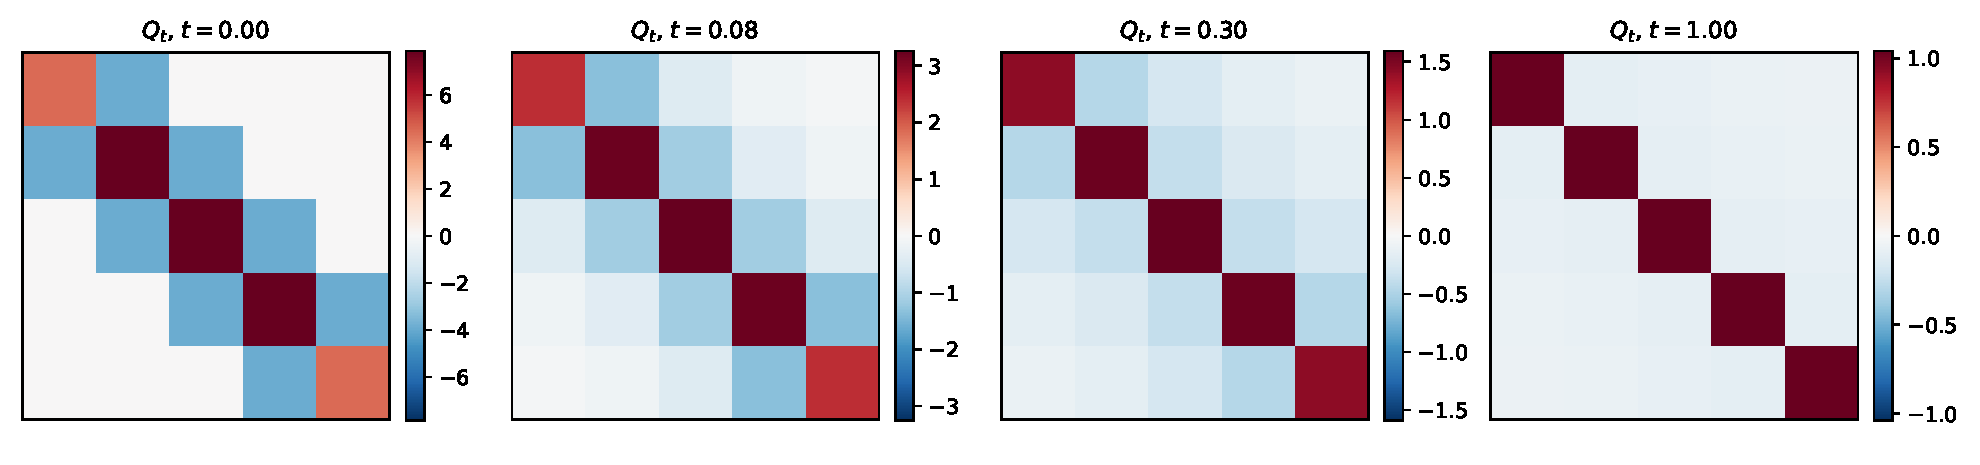
\includegraphics[width=.98\textwidth]{figures/fig02_small_fillin.pdf}
\caption{Small-$N$ heatmaps of $Q_t$ ($N=5$). At $t=0$ the matrix is exactly tridiagonal. For $t>0$ the zeros fill in immediately. The small matrix makes the first long-range entries visually obvious.}
\end{figure}

\begin{figure}[ht!]
\centering
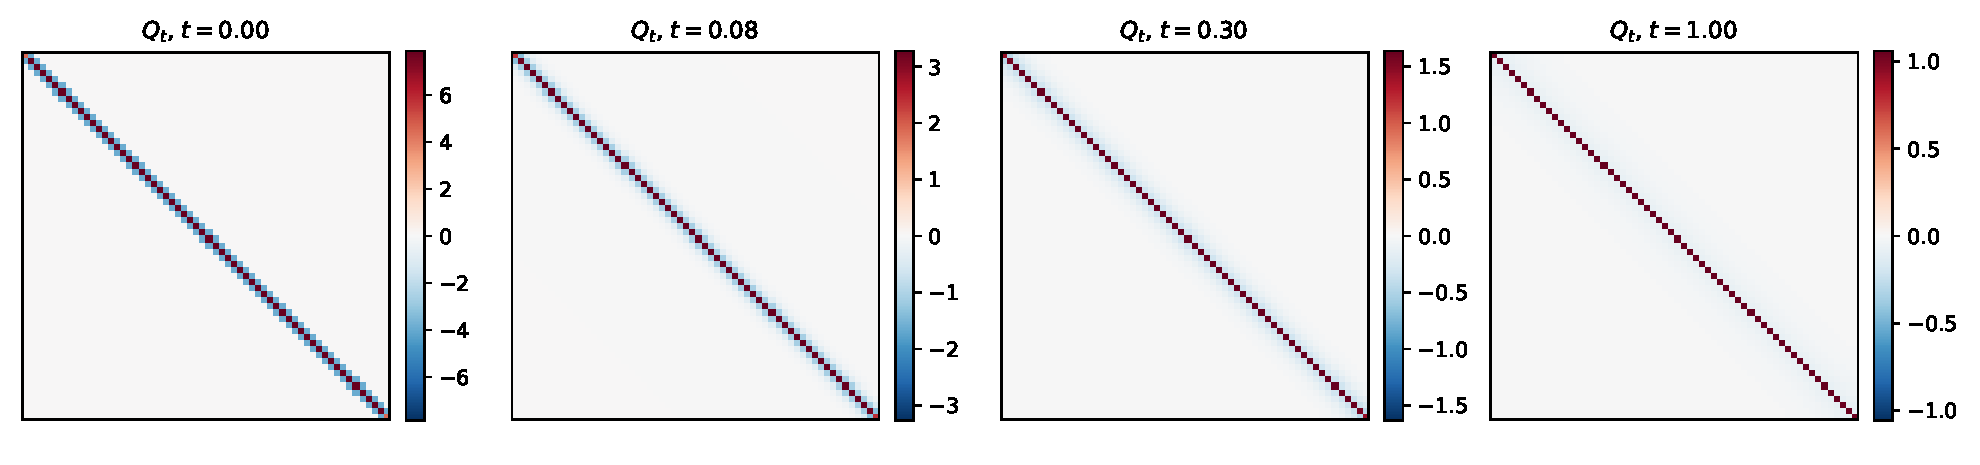
\includegraphics[width=.98\textwidth]{figures/fig03_large_fillin.pdf}
\caption{Large-$N$ heatmaps of $Q_t$ ($N=60$). The fill-in persists at scale: diffusion creates a full matrix whose entries are strongest near the diagonal and then decay away from it.}
\end{figure}

\begin{figure}[ht!]
\centering
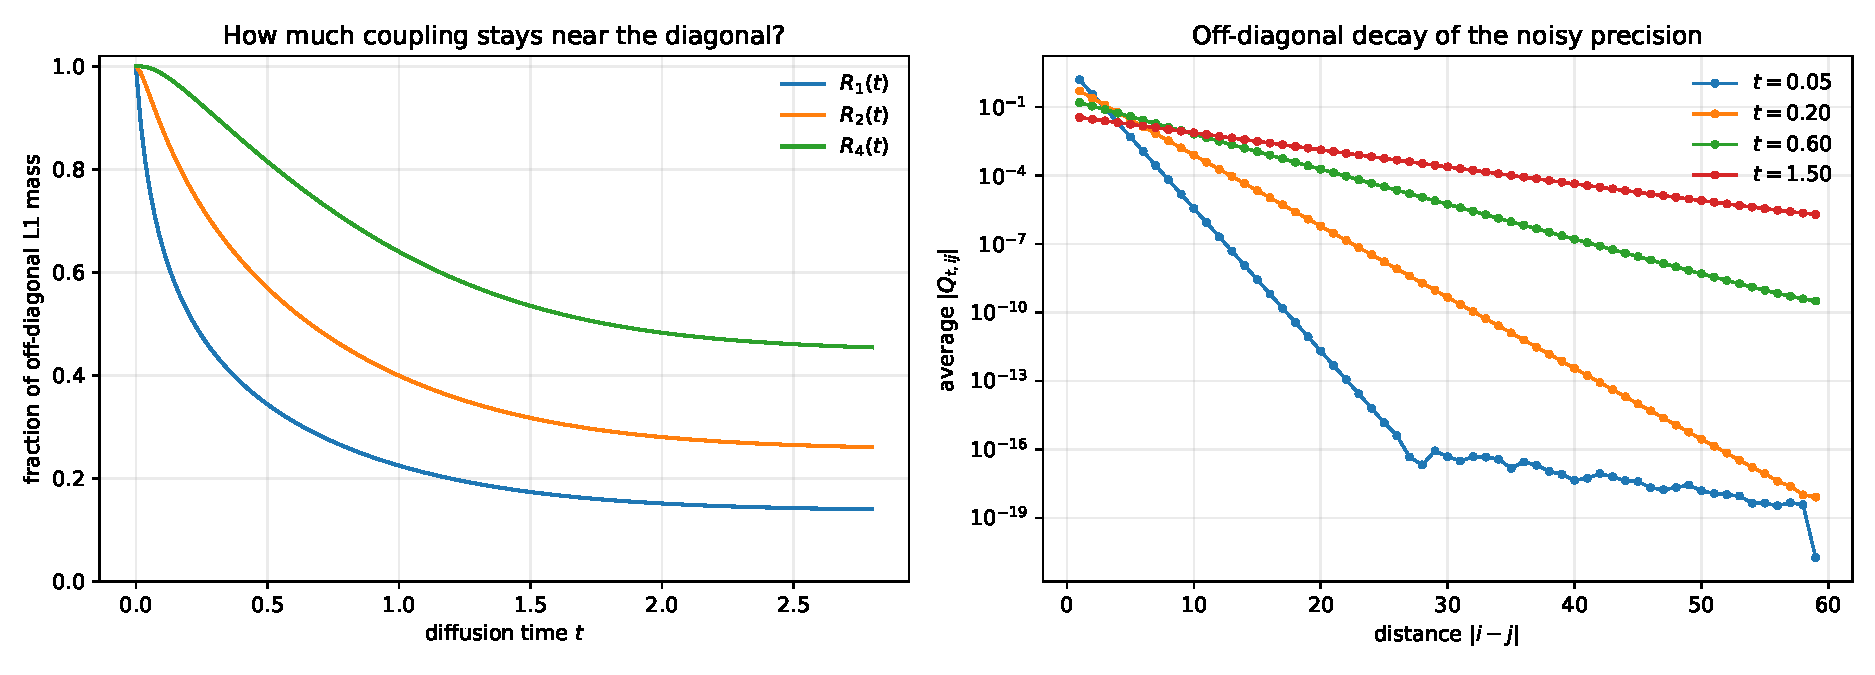
\includegraphics[width=.98\textwidth]{figures/fig04_metrics.pdf}
\caption{Left: nearest-band mass fractions $R_r(t)$ defined in \eqref{eq:Rr_def}. As soon as $t>0$, some coupling leaves the nearest-neighbor band. Right: the averaged off-diagonal profile $C_d(t)$ defined in \eqref{eq:Cd_def}; the near-linear behavior on a semilog axis is the numerical signature of exponential decay.}
\end{figure}

\begin{figure}[ht!]
\centering
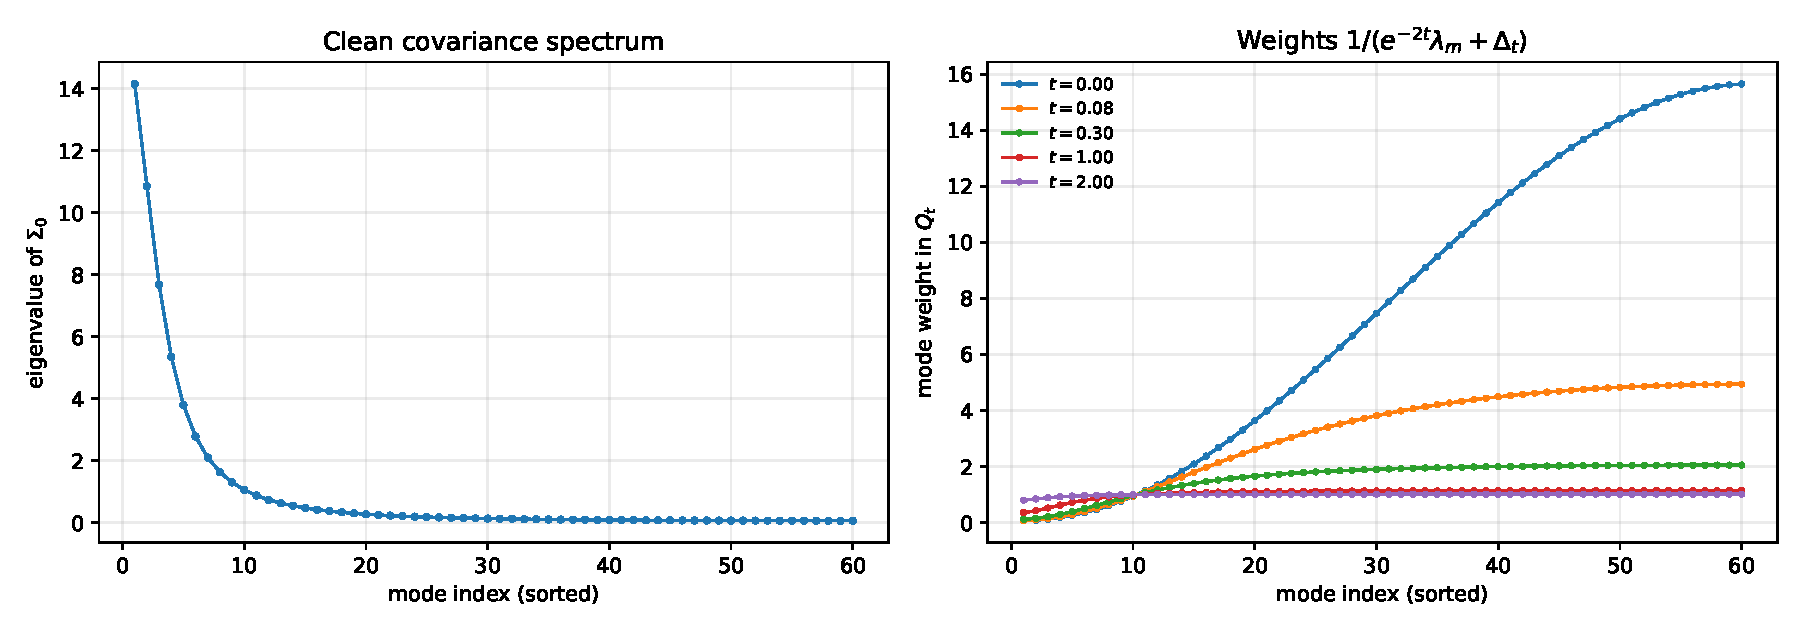
\includegraphics[width=.98\textwidth]{figures/fig05_spectrum.pdf}
\caption{Spectral picture. Left: clean covariance eigenvalues. Right: mode weights in the noisy precision. Diffusion changes the weights without changing the eigenvectors; this breaks the exact cancellation that made $Q_0$ tridiagonal.}
\end{figure}

The numerical results support the analytic picture exactly:
\begin{enumerate}[leftmargin=1.5em]
\item The clean matrix $Q_0$ is sparse because the Gaussian AR(1) chain is conditionally local.
\item The first positive diffusion time already creates nonzero long-range entries.
\item These long-range entries are not arbitrary: they decay rapidly with distance, consistent with \eqref{eq:qt_geometric}.
\item At late times the whole off-diagonal part collapses to zero and $Q_t$ approaches the identity.
\end{enumerate}

\section{Takeaway}
There are three distinct objects in play:
\[
\text{Markovianity} \quad \leftrightarrow \quad \text{sparse clean precision }Q_0,
\]
\[
\text{Gaussianity} \quad \leftrightarrow \quad \text{affine score }S(x,t)=-Q_t(x-\mu_t),
\]
\[
\text{diffusion} \quad \leftrightarrow \quad \text{change of inverse from }Q_0\text{ to }Q_t=(\beta_t\Sigma_0+\Delta_t\Id)^{-1}.
\]
The loss of Markovianity is therefore not mysterious. The clean covariance is dense, and matrix inversion is nonlocal. The exact tridiagonal zeros of $Q_0$ rely on a very specific cancellation. Diffusion perturbs the spectral weights, breaks that cancellation, and the zeros fill in. The resulting matrix remains structured---dense, but exponentially decaying---until isotropic noise eventually removes all coupling altogether.

\end{document}
